\documentclass[11pt]{article}
\usepackage{dsfont}
\usepackage[a4paper,margin = 0.6in, footskip = 0.1in, bottom= 1in, top=1.5in]{geometry}
\usepackage[utf8]{inputenc}
\usepackage{amsmath,amssymb,amsthm,bm}
\usepackage{tikz}
\usepackage{cite}
\usepackage{subfigure}
\usepackage{graphicx}
\usepackage{indentfirst}
\usepackage{url,booktabs}
\usepackage{multirow}
\usepackage{caption}
\usepackage{subcaption}
\usepackage{algpseudocode}
\usepackage{algorithm}
\usepackage{hyperref,xcolor}
\usepackage{natbib}
%\usepackage{romannum}
\newcommand{\RN}[1]{%
  \textup{\romannumeral#1}%
}

\begin{document}
\author{
\textbf{ESTATISTICA COMPUTACIONAL– ET591}\\
Grupo: Alan Gonçalves  e Arthur Machado\\
Exercícios - Lista 01
}
\date{Fevereiro, 2021}
\maketitle
\title{ }
* Os exercícios devem ser enviados em formato PDF e o correspondente documento em LateX, para ser compilado.
\begin{enumerate}
    \item Reproduza a escrita do seguinte texto:\\
    \begin{tikz}
\draw [dashed] (2,0) -- (19,0);
\end{tikz}

\section{Introduction}
For count data, overdispersion is not uncommon because the occurrence of zero counts might be greater than expected under the Poisson assumption. In this case, a zero inflated Poisson distribution should be more suitable to model the innovations. The zero inflated Poisson model has been widely used in many disciplines, including manufacturing applications, medicine, public health, environmental sciences, agriculture, among others.

To the best of our knowledge, there are no studies related to the analysis of data sets with excess of zeros and dependence structure with order larger than one, in both frequentist and Bayesian approaches.\\
To deal with this situation we propose an extension of the $\mathrm{INAR}(p)$ model, with zero-inflated Poisson innovations, called the $\mathrm{ZINAR}(p)$ model, for the analysis of count series with excess of zeros and time dependence with order larger than one. A Bayesian approach is conducted by developing an efficient MCMC algorithm to proceed the estimation of the parameters in the model. The performance is demonstrated by simulated and an original real data sets.

It’s important to emphasize that, the inference from the Bayesian perspective may result in richer inferences than does the likelihood-based approach in the case of small samples.

\subsection{The likelihood function}
Let $Y_1, \dots, Y_{n+p}, n>p$, be samples from the $\mathrm{ZINAR}(p)$ process. Denote the vector of all unknown parameters by $\boldsymbol{\theta} = (\boldsymbol{\alpha}, \rho, \lambda)$, where $\boldsymbol{\alpha} = (\alpha_{1}, \alpha_{2}, \dots, \alpha_{p})$. We further denote the joint pmf of $Y_{t-1}, \dost, Y_{n+p}$ given $\boldsymbol{\theta}$ by $\pi(y_1, \dots, y_{n+p}|\boldsymbol{\theta})$. Then, the likelihood function can be written as
\\
\begin{equation}
\pi(\boldsymbol{y}|\boldsymbol{\theta}) = \pi(y_1, \dots, y_p|\boldsymbol{\theta}) \prod_{t = p +1}^{p+n}\pi\left(y_t|Y_{t-1} = y_{t-1}, \dots, Y_{t-p} = y_{t-p}, \boldsymbol{\theta}\right),
\end{equation}
where
\begin{eqnarray}
\pi(y_t|Y_{t-1} = y_{t-1}, \dots, Y_{t-p} = y_{t-p}, \boldsymbol{\theta}) &=& \sum_{k_1=0}^{\mathrm{min}\{y_{t-1},
y_{t}\}}\binom{y_{t-1}}{k_1}\alpha^{k1}_{1}(1-\alpha_{1})^{y_{t-1} - k_1}\nonumber\\
&\times& \sum_{k_2=0}^{\mathrm{min}\{y_{t-2},
y_{t} - k_1\}}\binom{y_{t-2}}{k_2}\alpha^{k2}_{2}(1-\alpha_{2})^{y_{t-2} - k_2}\nonumber\\
&\times& \vdots\nonumber\\
&\times& \sum_{k_1=0}^{\mathrm{min}\{y_{t-p},
y_{t} - k_1 \dots -k_{p-1}\}}\binom{y_{t-p}}{k_p}\alpha^{kp}_{p}(1-\alpha_{p})^{y_{t-p} - k_p}\nonumber\\
&\times& \left[\rho^{\mathbb{I}}_{\{0\}}(y_{t} - k_1\dots-k_p) + (1 +\rho)\dfrac{e^{-\lambda}\lambda^{y_{t} - k_1 \dots -k_p}}{[y_{t} - k_1 \dots -k_p]!}  \right].\nonumber\\
&&
\end{eqnarray}

\begin{tikz}
\draw [dashed] (2,0) -- (19,0);
\end{tikz}
\item Escreva as seguintes tabelas:\\
(a)
\begin{table}[H]
\centering
\label{tab:my-table}
\begin{tabular}{|l|l|l}
\cline{1-2}
Etapa  & Atividades &  \\ \cline{1-2}
\multirow{2}{*}{1} &
\begin{tabular}[c]{@{}l@{}}
\textbf{Duração:}  \color{blue}De Fevereiro/2021 a Junho/2022\\
- Estudo do processo\\
- Estimação dos parâmetros\\ 
- Participação em Seminários e Eventos
\end{tabular} & \\ 
\cline{2-2} & 
\begin{tabular}[c]{@{}l@{}}
- Revisão bibliográfica\\
- Estudo sobre processos dinâmicos
\end{tabular}   &  \\ \cline{1-2}
\multirow{2}{*}{2} &
\begin{tabular}[c]{@{}l@{}}
\textbf{Duração:} :  \color{blue}De Julho/2022 a Janeiro/2023\\ 
- Estimação dos parâmetros\\
- Participação em Seminários e Eventos
\end{tabular}   &  \\ \cline{2-2} & 
\begin{tabular}[c]{@{}l@{}}
- Artigo submetido para publicação em periódico com boa avaliação;
\\ - Participação em Seminários e Eventos
\end{tabular}   &  \\ \cline{1-2}
\end{tabular}
\end{table}
(b)
\begin{table}[H]
\centering
\begin{tabular}{clllll}
\hline
\multicolumn{1}{l}{}                 &            &                 & \multicolumn{3}{c}{MCMC summary} \\ \cline{4-6} 
\multicolumn{1}{l}{Model}            & Parameter  & Real Value      & MC Mean   & MC SD    & MC Cov    \\ \hline
\multirow{3}{*}{$\mathrm{ZINAR}(1)$} & $\alpha$   & $\mathbf{0.40}$ & 0.3817    & 0.0836   & $96.4\%$  \\
                                     & $\lambda$  & $\mathbf{2.00}$ & 2.0300    & 0.2935   & $95.6\%$  \\
                                     & $\rho$     & $\mathbf{0.25}$ & 0.2458    & 0.1000   & $97.4\%$  \\ \hline
\multirow{3}{*}{$\mathrm{ZINAR}(2)$} & $\alpha_1$ & $\mathbf{0.40}$ & 0.3752    & 0.0959   & $97.7\%$  \\
                                     & $\alpha_2$ & $\mathbf{0.20}$ & 0.2198    & 0.0934   & $98.0\%$  \\
                                     & $\lambda$  & $\mathbf{2.00}$ & 2.0608    & 0.2185   & $96.5\%$  \\
\multicolumn{1}{l}{}                 & $\rho$     & $\mathbf{0.25}$ & 0.2645    & 0.1417   & $98.5\%$  \\ \hline
\end{tabular}
\caption{Tabela 1: Artificial data sets. Summary of MCMC results based on 500 simulated samples from the $\mathrm{ZINAR}(p)$ process, for $p = 1, \dots, 4$ and $n = 80$.}
\label{tab:my-table}
\end{table}
\item Reproduza a escrita do texto com suas respectivas referências bibliográficas:

\textit{A popular approach to deal with count time series having a dynamic structure depending on their
past observations, is to consider the integer-valued autoregressive (INAR) process, as proposed by \cite{Alzaid1987} and \cite{McKenzie1998}, in which the process is established by considering a
Poisson distribution for the innovations. However, in some cases, the Poisson distribution may be
inappropriate because of the property of equal mean and variance. In this regard, \cite{Ristic2009} proposed a geometric first order integer-valued autoregressive process with geometric marginals based on a negative binomial thinning operator.}

For count data, overdispersion is not uncommon because the occurrence of zero counts might be greater
than expected under the Poisson assumption. In this case, a zero inflated Poisson distribution should
be more suitable to model the innovations. The zero inflated Poisson model has been widely used in many disciplines, including manufacturing applications \citep{Lambert1992}, medicine (\citeauthor{Bohning1999}, 1999), public health \citep{Zhou2000}, environmental sciences \citep{Agarwal2002}, agriculture (\cite{Hall2000}; Garay et al. (\citeyear{Garay2011}, \citeyear{Garay2015})), among others. To handle with excess of zeros in count time series, \cite{Jazi2015} introduced the stationary ZINAR(1) process with innovations having a zero-inflated Poisson distribution. The authors also showed that the marginal distribution of the process
is zero-inflated. Afterward, \cite{Barreto2015} defined a zero-modified geometric INAR(1) process, which is able to capture deflation or inflation of zeros as well as overdispersion and underdispersion.

\bibliographystyle{elsarticle-harv}
\bibliography{lista1referencias}

\item Represente, como nas figuras a seguir, os gráficos enviados:

\begin{figure}[H]
    \centering
    \caption{Graphical representations of the estimated copula at different levels - dependent components without thresholds.\\
    Last graphic is for the Normal copula.}
    \begin{subfigure}
    \centering
    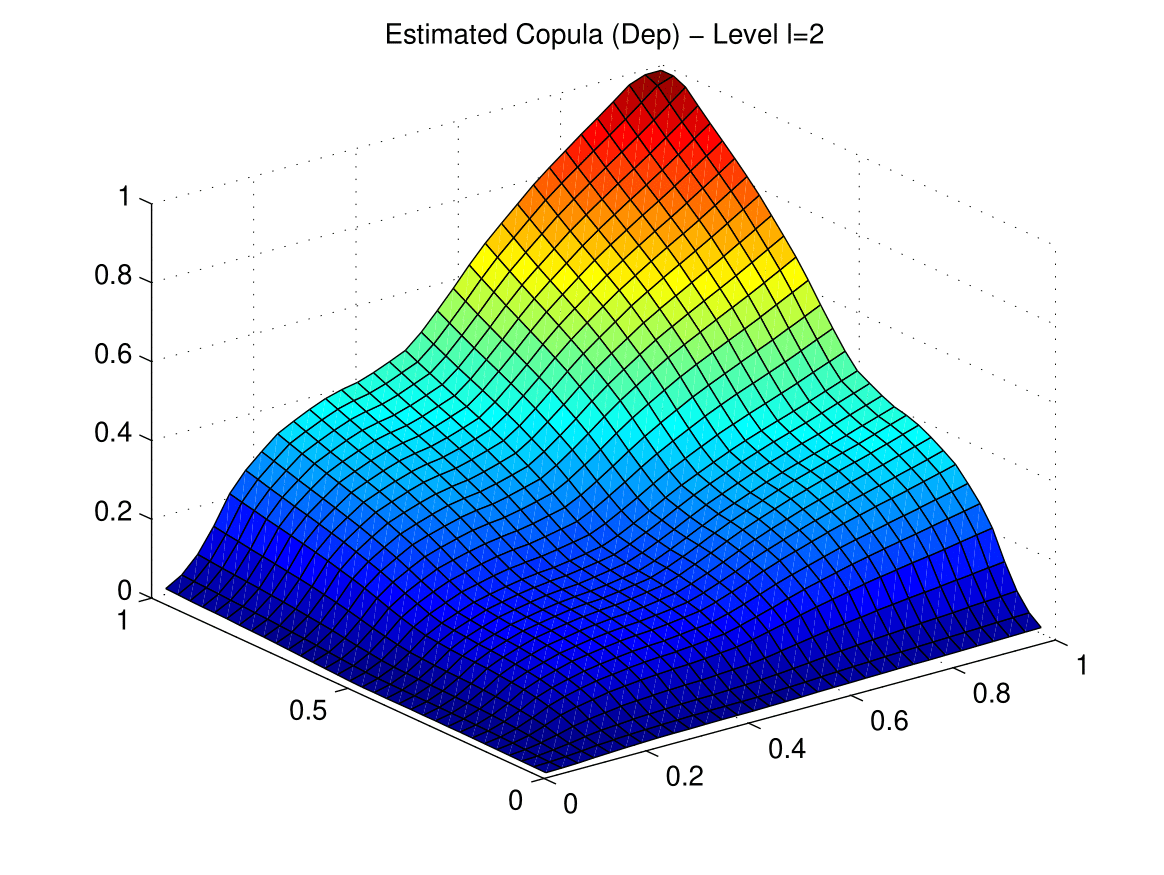
\includegraphics[width=7cm, height=6cm]{Figura1-1.png}
    \end{subfigure}
    \begin{subfigure}
    \centering
    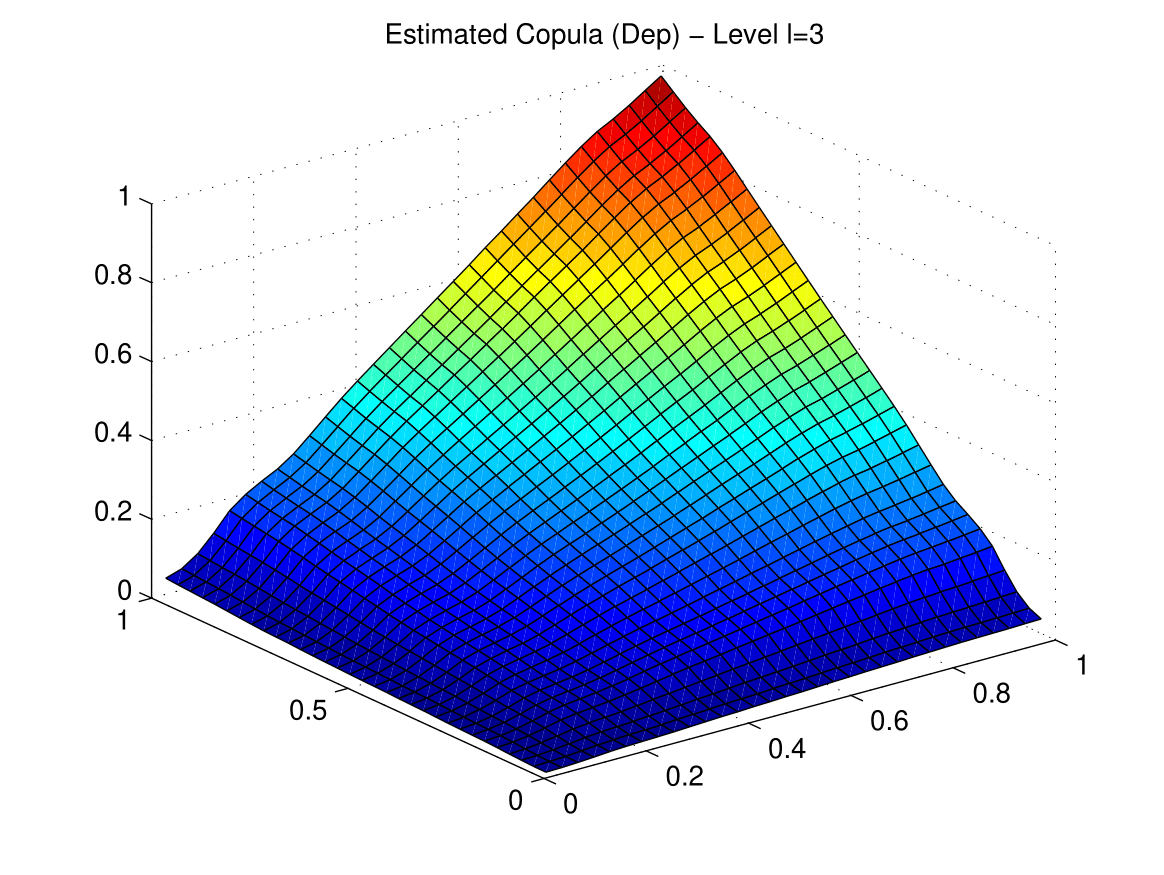
\includegraphics[width=7cm, height=6cm]{Figura2-1.png}
    \end{subfigure}
    
    \begin{subfigure}
    \centering
    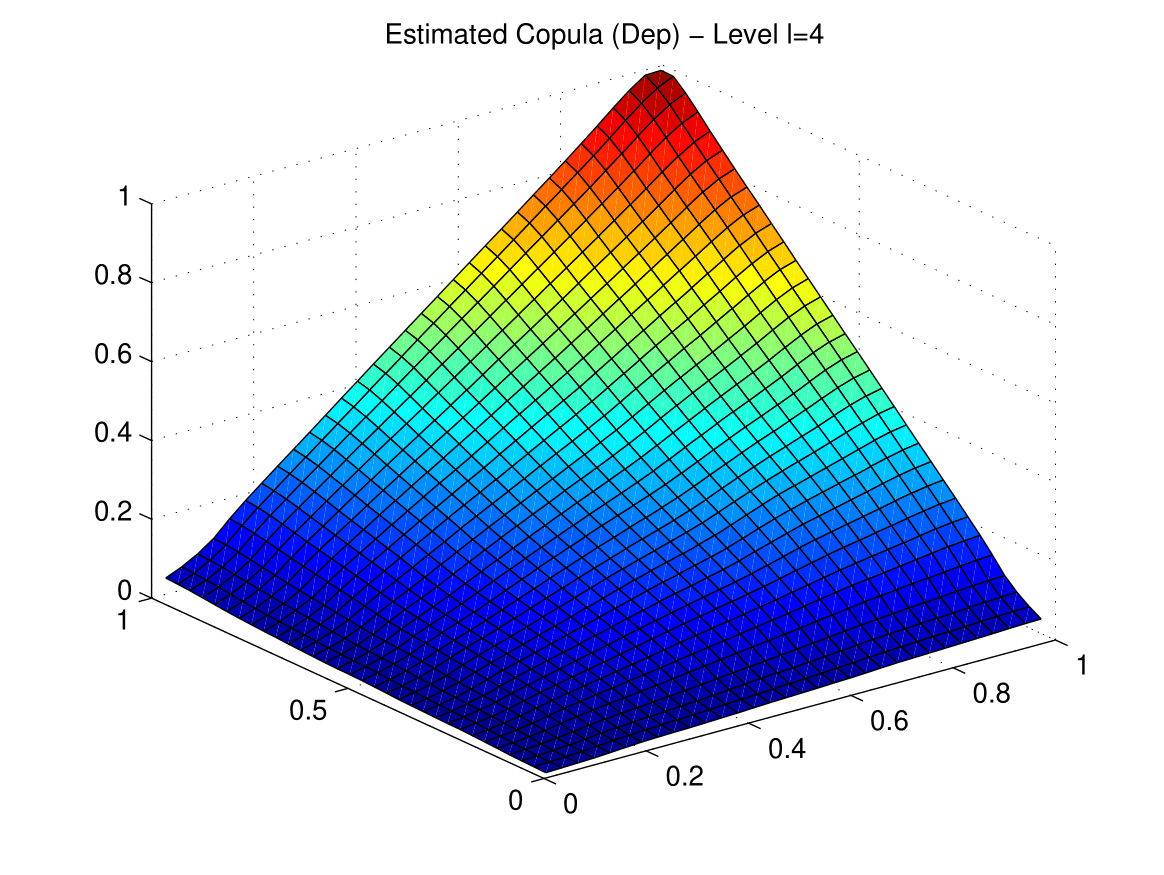
\includegraphics[width=7cm, height=6cm]{Figura3-1.png}
    \end{subfigure}
    \begin{subfigure}
    \centering
    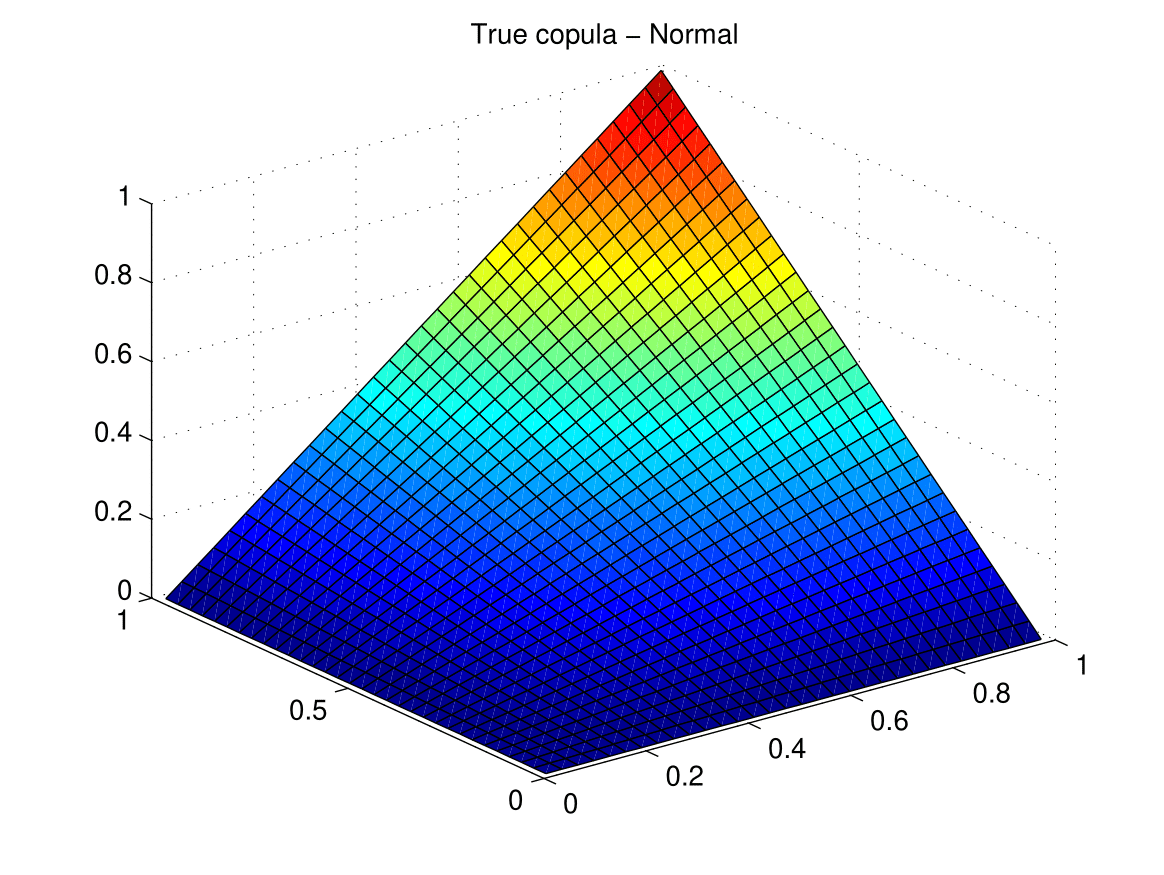
\includegraphics[width=7cm, height=6cm]{Figura4-1.png}
    \end{subfigure}


    \label{fig:copulagraph}
\end{figure}


\begin{figure}[H]
    \centering
    \begin{subfigure}
    \centering
    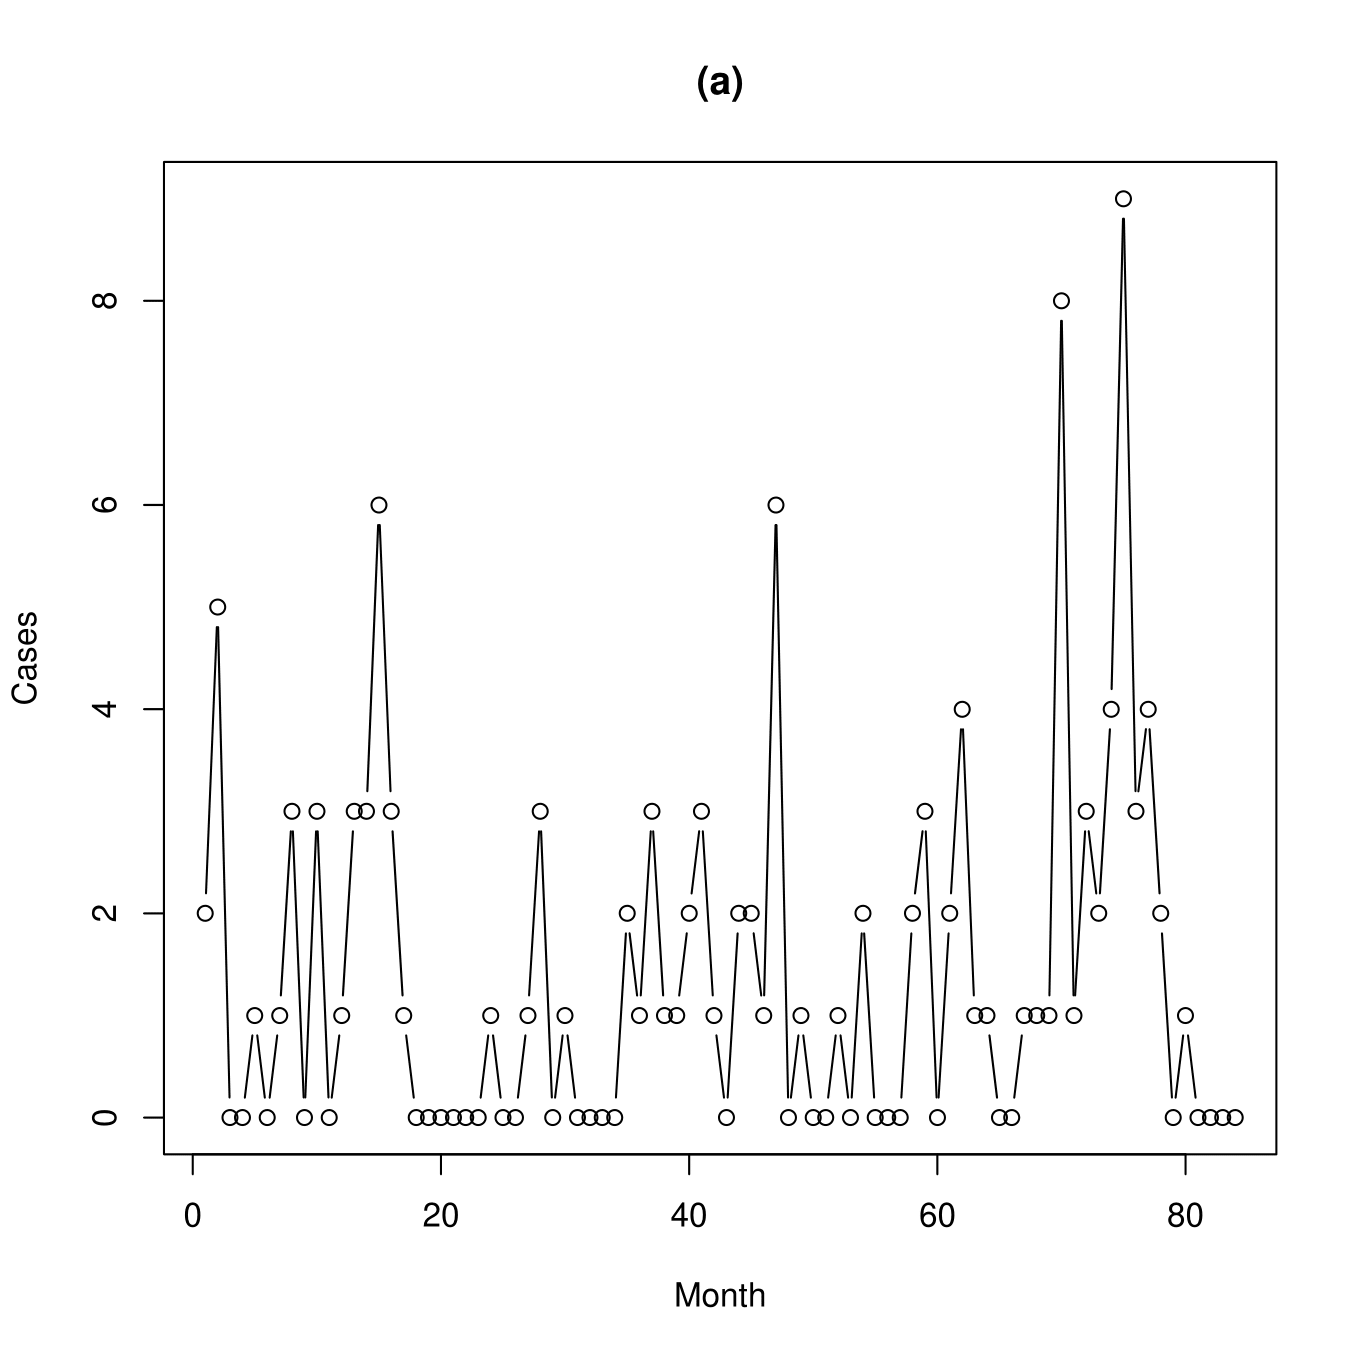
\includegraphics[width=7cm, height=6cm]{Slesion-1.png}
    \end{subfigure}
    \begin{subfigure}
    \centering
    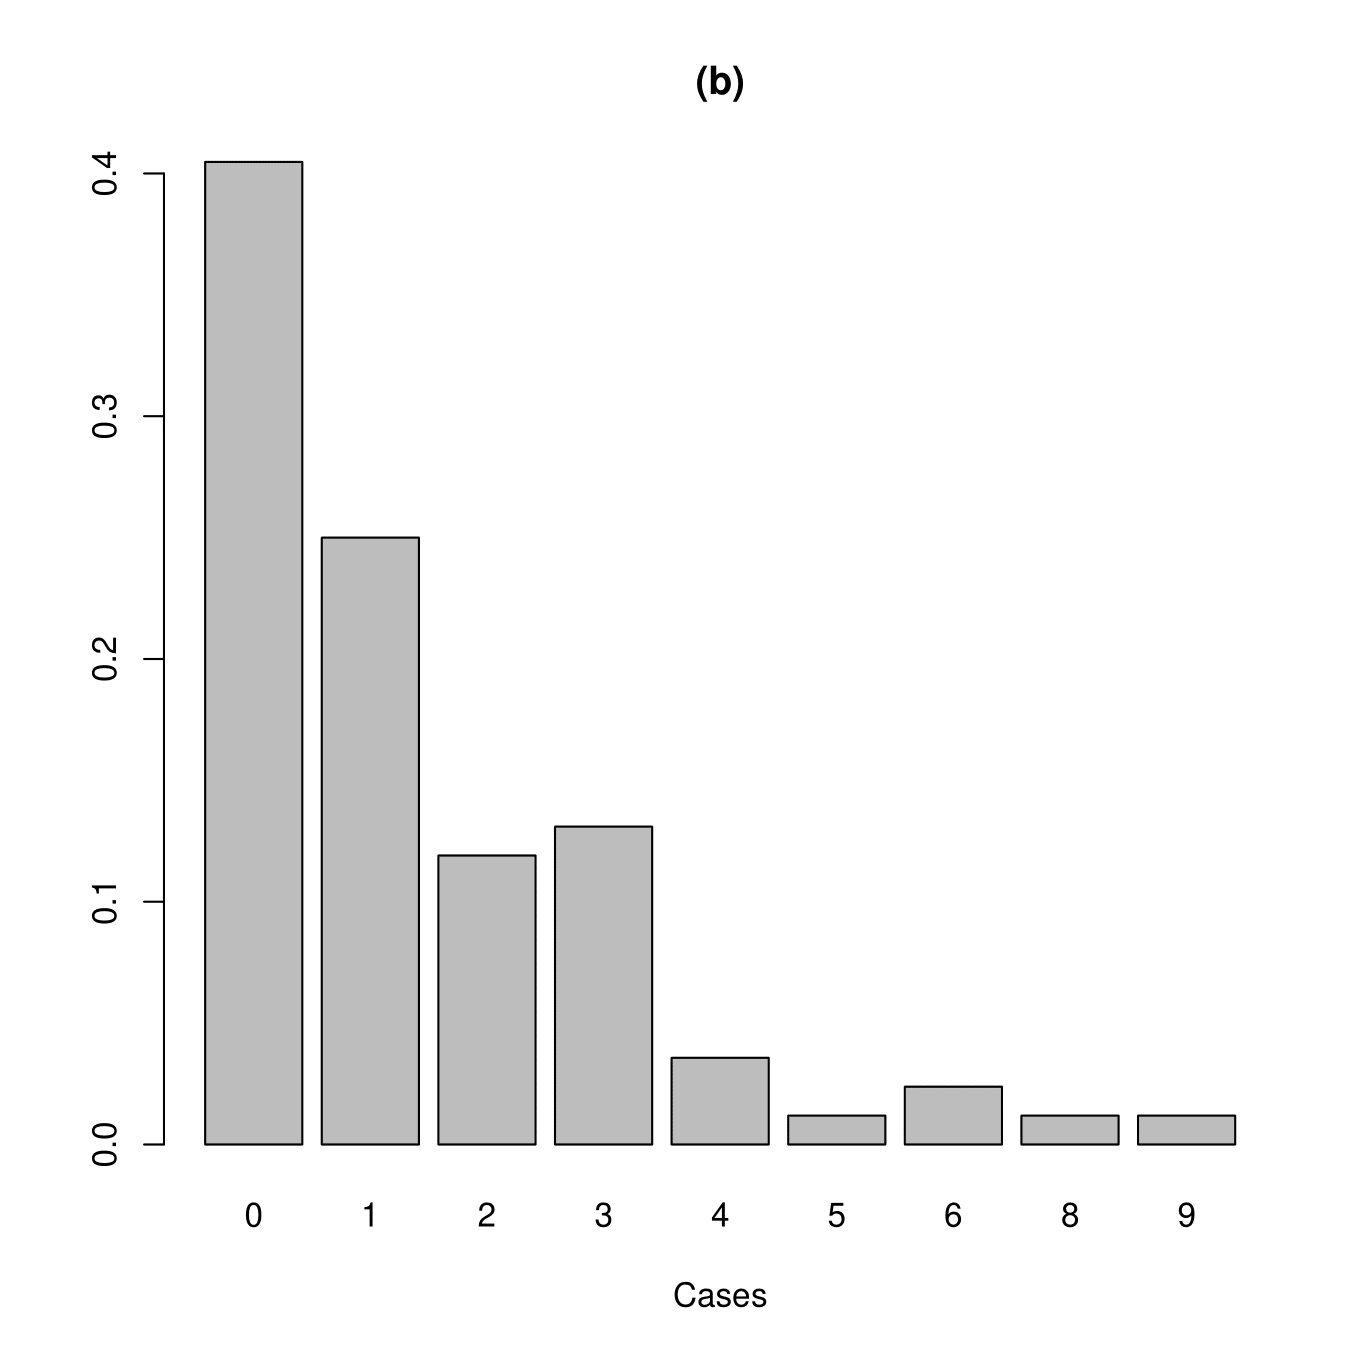
\includegraphics[width=7cm, height=6cm]{SlesionBarPlot-1.png}
    \end{subfigure}
    
    \begin{subfigure}
    \centering
    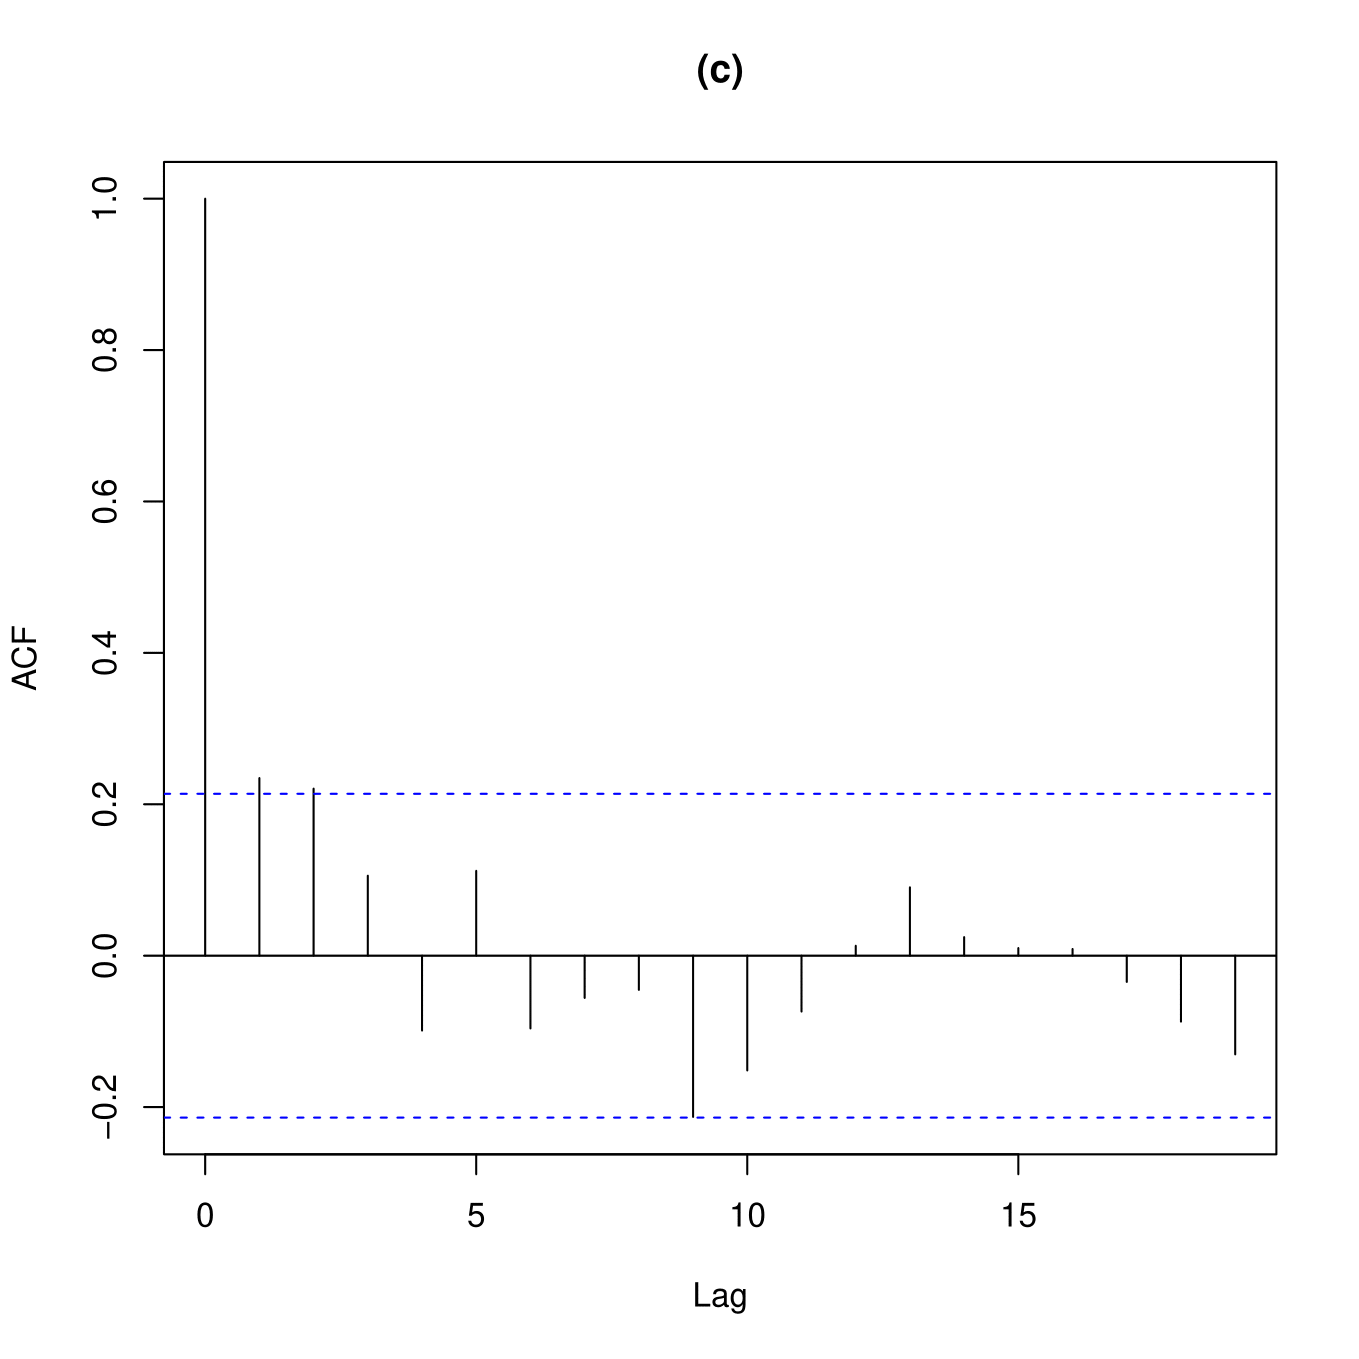
\includegraphics[width=7cm, height=6cm]{SlesionACF-1.png}
    \end{subfigure}
    
    \caption{Skin-lesions dataset. (a) Time Series. (b) Bar plot. (c)ACF}


    \label{fig:copulagraph}
\end{figure}

\end{enumerate}
\end{document}
